\documentclass[UTF8,a4paper]{ctexart}
\usepackage[utf8]{inputenc}
\usepackage{amsmath}
\usepackage{pdfpages}
\usepackage{graphicx}
\usepackage{wrapfig}
\usepackage{listings}
\title{线控作业1}
\author{张蔚桐\ 2015011493\ 自55}
\begin {document}
\maketitle
\section{}
文章主要探讨了利用频率响应作为检测传递函数的方法对硬盘控制系统的优化等问题,这里略去
\section{}
从图\ref{f1ori}中可以预计,系统的传递函数可以表示为$G(s)=\frac{K}{s(T_1s+1)(T_2s+1)},T_1>0,T_2>0$可以根据相频图估计转折频率$\omega_1=18.14\rm{rad/s},\omega_2=1103\rm{rad/s}$可得$T_1=\frac{1}{\omega_1}=0.551\rm{s},T_2=\frac{1}{\omega_2}=0.9066\times 10^{-3}\rm{s}$,同时,考虑辐频在$\omega=1\rm{rad/s}$附近的增益可得$20lg(K)=-9.2;K=0.346$因此系统传递函数可以表示为$$G(s)=\frac{0.346}{s(0.551s+1)(0.9066\times 10^{-3}s+1)}$$,对应的Bode图如图\ref{f1the}所示,可以看出和实际bode图\ref{f1ori}还是基本符合的
\begin{figure}
\centering
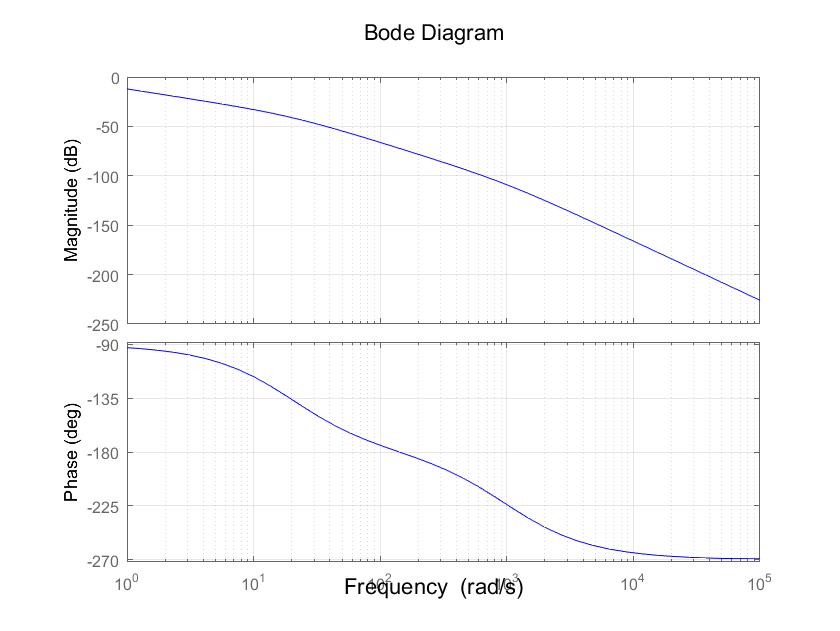
\includegraphics[width=\textwidth]{motorG.jpg}
\caption{原图像}
\label{f1ori}
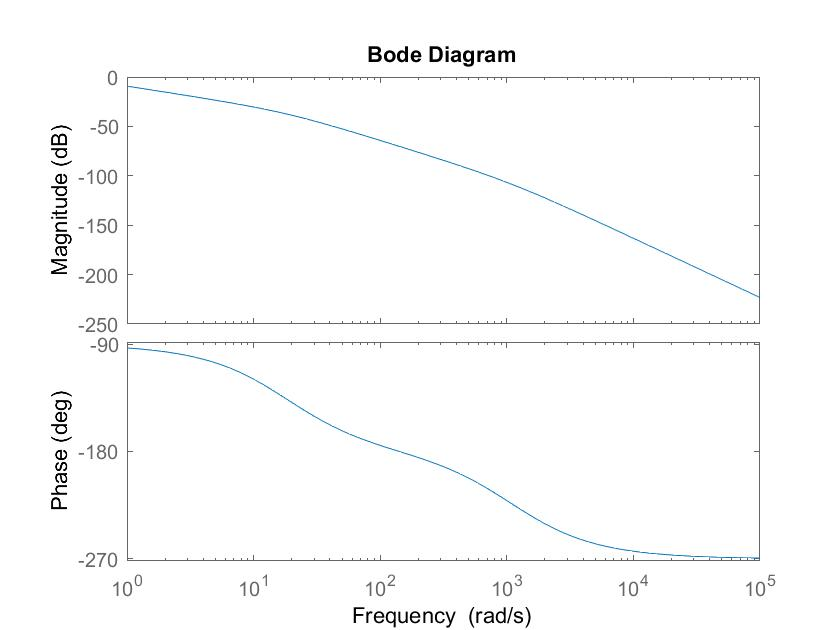
\includegraphics[width=\textwidth]{RmotorG.jpg}
\caption{理论图像}
\label{f1the}
\end{figure}
\section{}
如图\ref{f2ori}显然这是一个惯性环节的图像,可以直接看出$$G(s)=\frac{0.102}{(0.001s+1)}$$MATLAB仿真之后的图像如图\ref{f2the}所示,和原图\ref{f2ori}基本一致
\begin{figure}
\centering
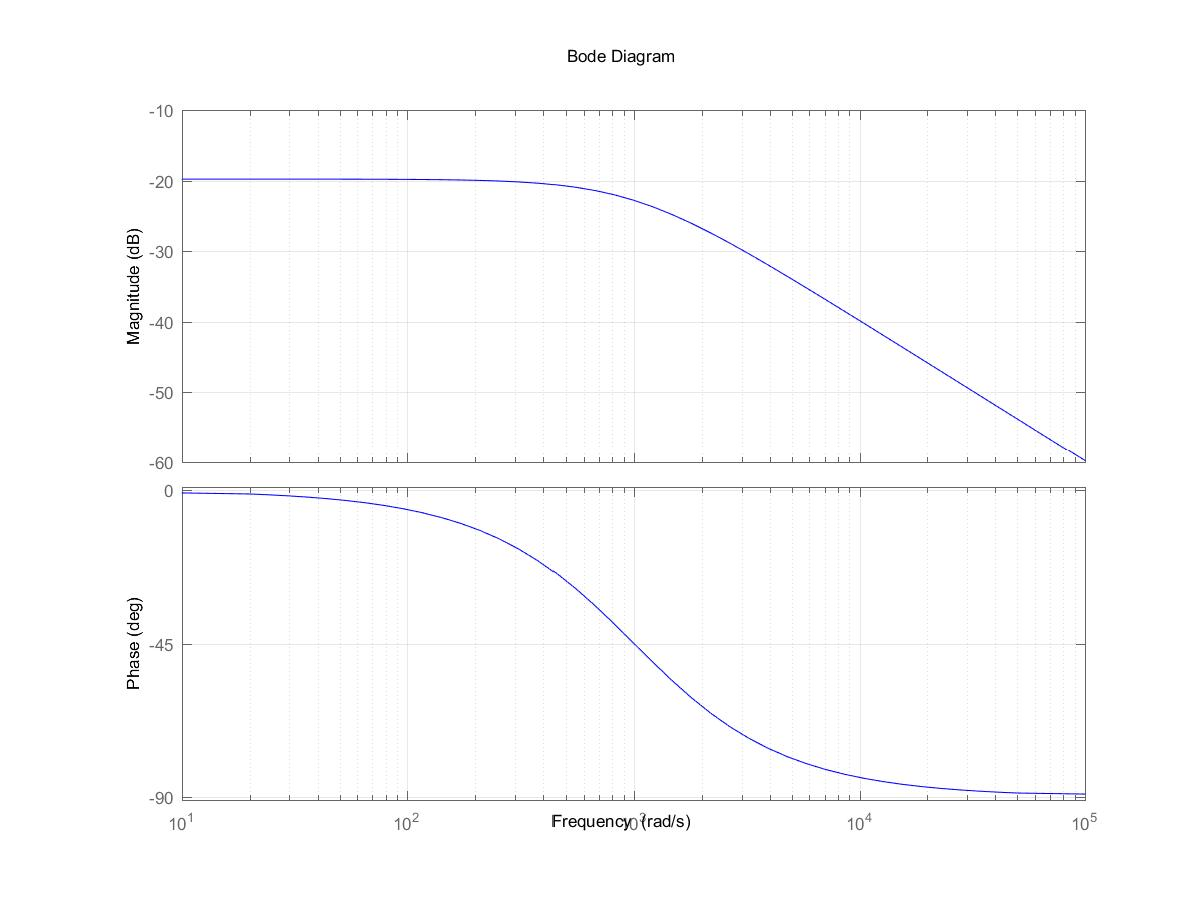
\includegraphics[width=\textwidth]{motorG1.jpg}
\caption{原图像}
\label{f2ori}
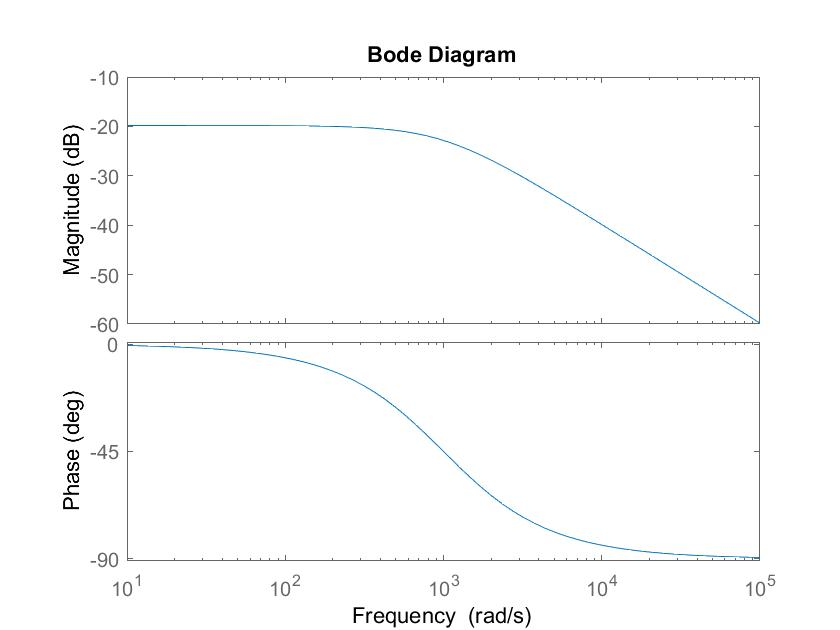
\includegraphics[width=\textwidth]{RmotorG1.jpg}
\caption{理论图像}
\label{f2the}
\end{figure}
\section{}
可以看出系统的传递函数为$G(s)=\frac{K}{s(Ts+1)},T>0$,并由图\ref{f3ori}可以得到$20lg(K)=7.196,K=2.29,T=\frac{1}{20}=0.05$因此$$G(s)=\frac{2.29}{s(0.05s+1)}$$MATLAB作图如图\ref{f3the}所示,和实际情况相差不多
\begin{figure}
\centering
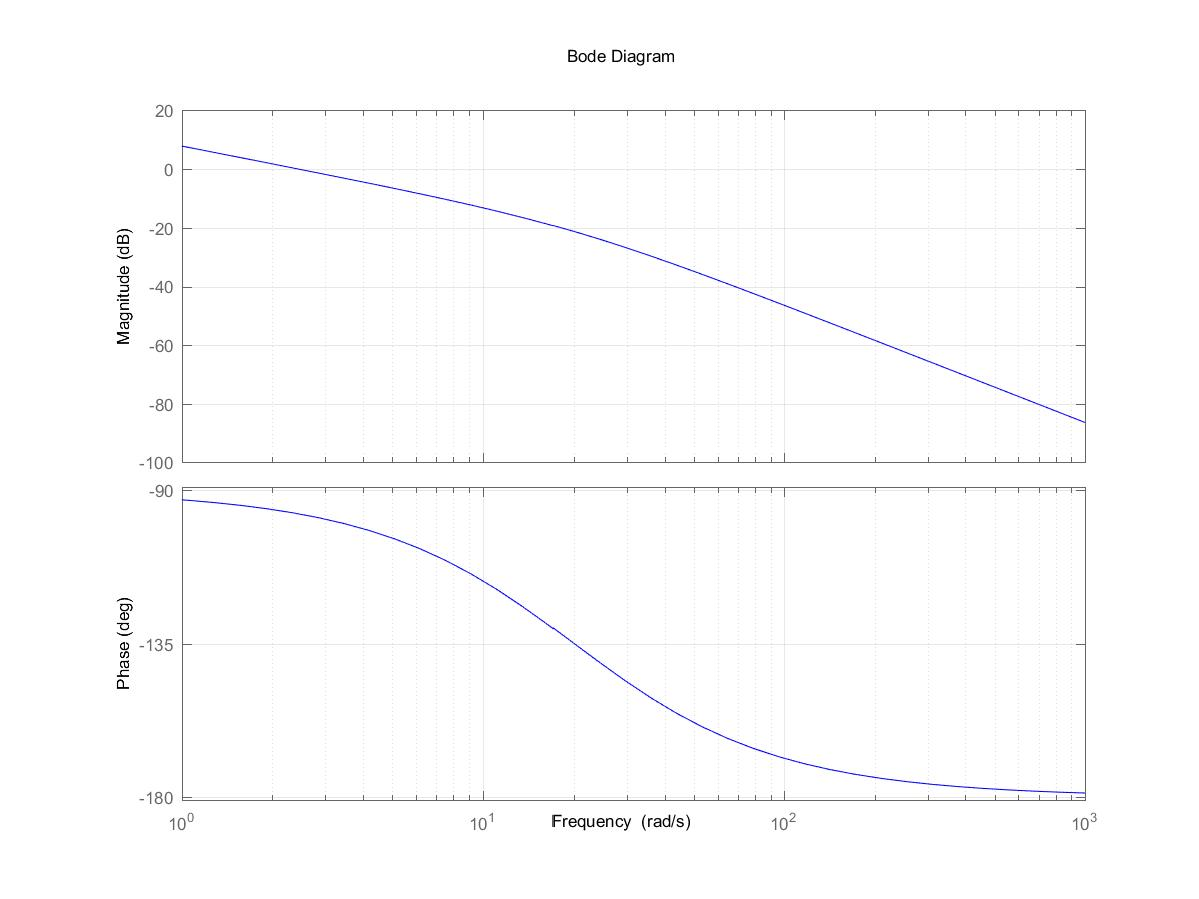
\includegraphics[width=\textwidth]{motorG2.jpg}
\caption{原图像}
\label{f3ori}
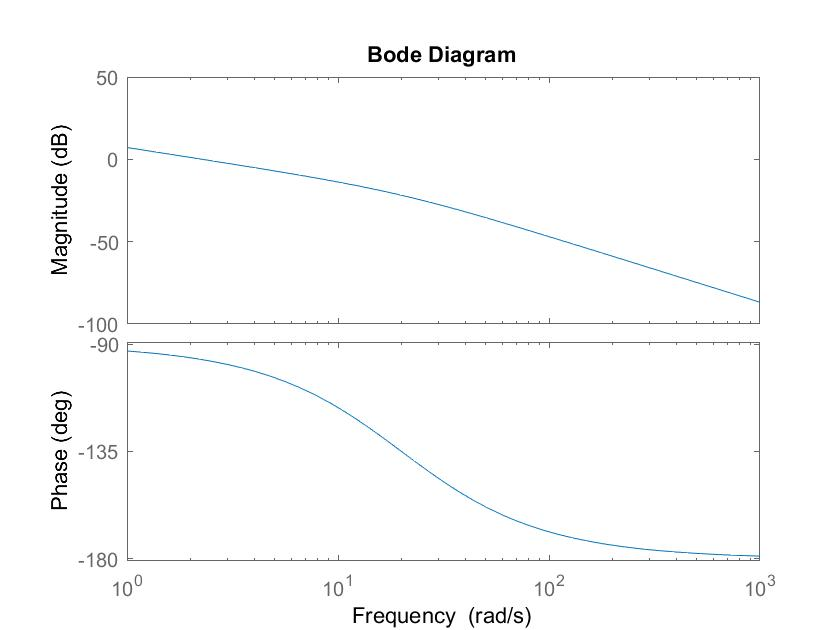
\includegraphics[width=\textwidth]{RmotorG2.jpg}
\caption{理论图像}
\label{f3the}
\end{figure}
\section{}
根据KCL,KVL,可以得到
$$\begin{cases}
\dot{x_3}=\frac{1}{C_3}x_4 \\
\dot{x_4}=-\frac{1}{L_1}x_1-\frac{1}{L_1}x_3+\frac{1}{L_1}u \\
\dot{x_2}=-\frac{1}{C_2R}x_1-\frac{1}{C_2R}x_2+\frac{1}{C_2R}u \\
\dot{x_1}=\frac{1}{C_1}x_4-\frac{C_2}{C_1}\dot{x_2} = \frac{1}{C_1R}x_1+\frac{1}{C_1R}x_2+\frac{1}{C_1}x_4-\frac{1}{C_1R}u
\end{cases}$$
并进一步得到$$y=RC_2\dot{x_2}=-x_1-x_2+u$$因此得到
$$\begin{cases}

\mathbf{A}=\begin{pmatrix}
\frac{1}{RC_1} & \frac{1}{RC_1} & 0 & \frac{1}{C_1} \\
-\frac{1}{RC_2} & -\frac{1}{RC_2} & 0 & 0 \\
0 & 0 & 0 & \frac{1}{C_3} \\
-\frac{1}{L_1} & 0 & -\frac{1}{L_1} & 0
\end{pmatrix} ;
\mathbf{b}=\begin{pmatrix}
-\frac{1}{RC_1} &
\frac{1}{RC_2} &
0 &
\frac{1}{L_1}
\end{pmatrix}^\mathbf{T}\\
\\ 
\mathbf{c}^\mathbf{T}=\begin{pmatrix}
-1 & -1 & 0 & 0 \end{pmatrix};
\mathbf{d}=\begin{pmatrix} 1 \end{pmatrix}
\end{cases}$$
\section{}
由泊肃叶定律,可以得到状态方程为 $$\begin{cases}
c_1x_1=u_1+\frac{\rho g}{R_2}x_2-\frac{\rho g}{R_2}x_1-\frac{\rho g}{R_1}x_1 \\
c_2x_2=u_2-\frac{\rho g}{R_2}x_2+\frac{\rho g}{R_2}x_1\end{cases}$$
输出方程为$$y=\frac{\rho g}{R_1}x_1$$其中$\rho$是液体的密度,$g$是重力加速度
\section{}
记滑块1的位置为$F_1$滑块2的位置为$F_2$,由牛顿第二定律得$$\begin{cases}
m_2\ddot{F_2}=u(t)+k(F_1-F_2-l)-\xi_2\dot{F_2} \\
m_1\ddot{F_1}=-k(F_1-F_2-l)-\xi_1\dot{F_1}
\end{cases}$$
于是可以处理得到$$\begin{cases}
m_2F_2s^2=U(s)+kF_1-kF_2-\xi F_2 s \\
m_1F_1s^2=-kF_1+kF_2-\xi_1 F_1s
\end{cases}$$
于是$$(m_1s^2+\xi_1s+k)F_1=k\frac{U(s)+kF_1}{m_2s^2+\xi_2s+k}$$
整理得到$$G(s)=\frac{k}{(m_1s^2+\xi_1s+k)(m_2s^2+\xi_2s+k)-k^2}$$
状态方程采用更简单的方式求取,设弹簧压缩的长度为$x_3$,两个物体的速度为$x_1,x_2$第1个物体的位移是$x_4$,由牛顿力学可得$$\begin{cases}
m_1\dot{x_1}=-\xi_1x_1+kx_3 \\
m_2\dot{x_2}=-\xi_2x_2-kx_3+u \\
\dot{x_3}=x_2-x_1 \\
\dot{x_4}=x_1  \end{cases}$$
于是得到$$\begin{cases}
\mathbf{A}=\begin{pmatrix}
-\frac{\xi_1}{m_1} & 0 & \frac{k}{m_1} & 0\\
0 & \frac{\xi_2}{m_2} & -\frac{k}{m_2} & 0\\
-1 & 1 & 0 & 0\\
1 & 0 & 0 & 0 \end{pmatrix} ;
\mathbf{b}=\begin{pmatrix} 0& 1& 0 & 0\end{pmatrix}^\mathbf{T} \\ \\ 
\mathbf{c^T}=\begin{pmatrix} 0& 0&0&1 \end{pmatrix} ;
\mathbf{d}=0\end{cases}$$
\section{}
$$\begin{cases}
\mathbf{A}=\begin{pmatrix} 0& 1\\ \frac{g}{l} & 0 \\ \end{pmatrix};
\mathbf{b}=\begin{pmatrix} 0& 1\end{pmatrix}^T\end{cases}$$
\section{}
设$\dddot{x}+7\ddot{x}+14\dot{x}+8x=u$
同时$$\begin{cases} x_1=x \\ x_2=\dot{x} \\ x_3=\ddot{x} \end{cases}$$
于是得到$$\begin{cases}
\mathbf{A}=\begin{pmatrix} 
0 & 1 & 0 \\
0 & 0 & 1  \\
-8& -14& -7 \end{pmatrix} ;
\mathbf{b}=\begin{pmatrix} 0 & 0 & 1 \end{pmatrix}^\mathbf{T}\\ \\
\mathbf{c^T}=\begin{pmatrix} 3 & 0 & 0 \end{pmatrix} ;
\mathbf{d}=0 \end{cases}$$
考察实现,传递函数可以化为
$$\frac{Y(s)}{U(s)}=\frac{3s^{-3}}{1+7s^{-1}+14s^{-2}+8s^{-3}}$$记$$e(s)=\frac{u(s)}{(1+7s^{-1}+14s^{-2}+8s^{-3})}$$
于是得到
$$\begin{cases}Y(s)=3s^{-3}e(s)\\ e(s)=u(s)-7s^{-1}e(s)-14s^{-2}e(s)-8s^{-3}e(s)\end{cases}$$可以得到模拟电路图
如图\ref{simu1}为其模拟结构图
\begin{figure}
\centering
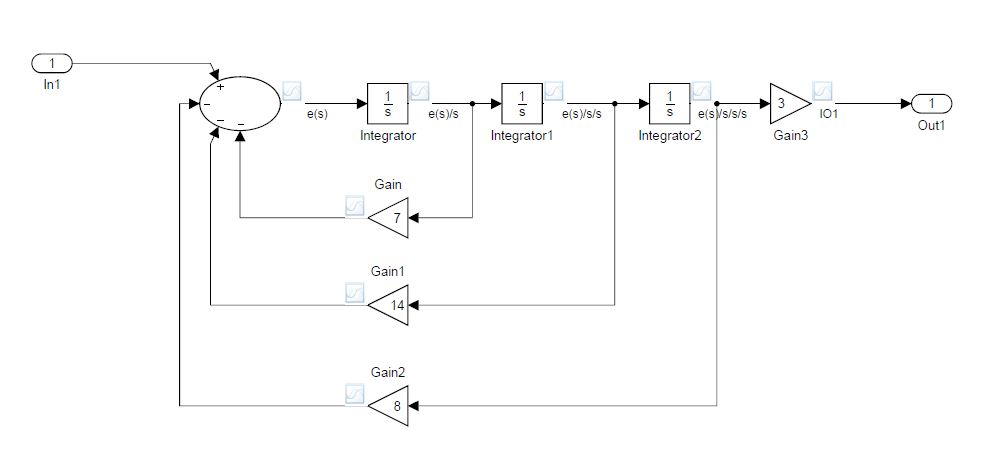
\includegraphics[width=\textwidth]{Simu1.JPG}
\caption{10.模拟结构图}
\label{simu1}
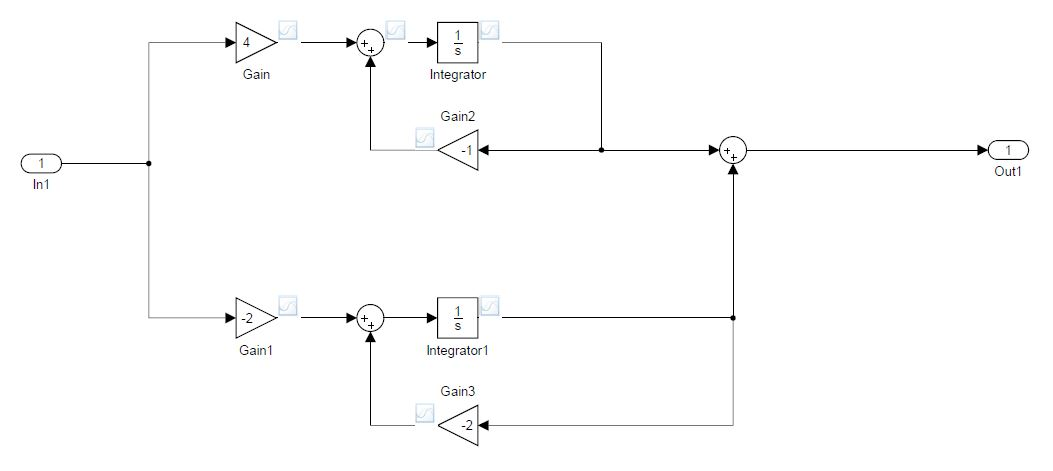
\includegraphics[width=\textwidth]{Simu2.JPG}
\caption{11.模拟结构图}
\label{simu2}
\end{figure}
\section{}
显然$$G(s)=\frac{4}{s+1}+\frac{-2}{s+2}$$于是可以得到其系统结构图\ref{simu2}并进一步可以得到解耦标准型:$$\begin{cases}
\mathbf{A}=\begin{pmatrix} -1 & 0 \\ 0 & -2 \end{pmatrix},
\mathbf{b}=\begin{pmatrix} 4 & -2 \end{pmatrix}^{\mathbf{T}} \\ \\
\mathbf{c^T}=\begin{pmatrix} 1 & 1 \end{pmatrix},
\mathbf{d}=0 \end{cases}$$
\section{}
\subsection{}
$$\begin{cases}
\mathbf{A}=\begin{pmatrix}
0&1&0&0\\
-2&-3&0&0\\
0&0&0&1\\
0&0&-4&-4\end{pmatrix};
\mathbf{b}=\begin{pmatrix} 0&1&0&1\end{pmatrix}^\mathbf{T} \\ \\ 
\mathbf{c}^\mathbf{T}=\begin{pmatrix} 1&0&1&2\end{pmatrix};
\mathbf{d}=0 \end{cases} $$
\subsection{}
$$\begin{cases}
\mathbf{A}=\begin{pmatrix}
0&1&0&0\\
-2&-3&0&0\\
0&0&0&1\\
1&0&-4&-4\end{pmatrix},
\mathbf{b}=\begin{pmatrix} 0&1&0&0\end{pmatrix}^\mathbf{T} \\ \\ 
\mathbf{c}^\mathbf{T}=\begin{pmatrix} 0&0&1&2\end{pmatrix}, 
\mathbf{d}=0 \end{cases} $$
\subsection{}
$$\begin{cases}
\mathbf{A}=\begin{pmatrix}
0&1&0&0\\
-2&-3&-1&-2\\
0&0&0&1\\
1&0&-4&-4\end{pmatrix},
\mathbf{b}=\begin{pmatrix} 0&1&0&0\end{pmatrix}^\mathbf{T} \\ \\ 
\mathbf{c}^\mathbf{T}=\begin{pmatrix} 1&0&0&0\end{pmatrix},
\mathbf{d}=0 \end{cases} $$
\section{}
$$G(s)=\begin{pmatrix} 1&1&1\\ -2&-3&-4\end{pmatrix}
\begin{pmatrix} s+2&0&0\\ 0&s+3&0\\ 0&0&s+4 \end{pmatrix}^{-1}
\begin{pmatrix} 1&-1\\ -5&4\\ 5&-3\end{pmatrix} $$ $$G(s) = \begin{pmatrix} \frac{1}{s+2}&\frac{1}{s+3}&\frac{1}{s+4}\\ \frac{-2}{s+2}&\frac{-3}{s+3}&\frac{-4}{s+4}\end{pmatrix}
\begin{pmatrix} 1&-1\\ -5&4\\ 5&-3\end{pmatrix}$$
$$G(s)=\begin{pmatrix} 
\frac{1}{s+2}-\frac{5}{s+3}+\frac{5}{s+4} & -\frac{1}{s+2}+\frac{4}{s+3}-\frac{3}{s+4} \\
-\frac{2}{s+2}+\frac{10}{s+3}-\frac{20}{s+4} & \frac{2}{s+2}-\frac{12}{s+3}+\frac{12}{s+4} \end{pmatrix}$$
\section{}
$$\begin{cases}
\dot{x_1}=-2x_1-50x_2-50x_3+10u\\
\dot{x_2}=x_1+x_4+x_2+x_3\\
\dot{x_3}=x_1+x_4+x_2\\
\dot{x_4}=-x_2-x_3+3x_4
\end{cases}$$
于是得到
$$\begin{cases}
\mathbf{A}=\begin{pmatrix}
-2&-50&-50&0\\
1&1&1&1\\
1&1&0&1\\
0&-1&-1&3\end{pmatrix},
\mathbf{b}=\begin{pmatrix} 0&0&0&10\end{pmatrix}^\mathbf{T} \\ \\ 
\mathbf{c}^\mathbf{T}=\begin{pmatrix} 0&1&1&0\end{pmatrix},
\mathbf{d}=0 \end{cases} $$
\section{}
显然有$$\mathbf{x}=\begin{pmatrix}
\mathrm{e}^{2t} & t\mathrm{e}^{2t} & \frac{t^2}{2}\mathrm{e}^{2t} \\
0 & \mathrm{e}^{2t} & t\mathrm{e}^{2t} \\
0 &0 & \mathrm{e}^{2t} 
\end{pmatrix}\mathbf{x_0},where\  \mathbf{x_0}=(x_1(0),x_2(0),x_3(0))^{\rm{T}}$$
\section{}
$$\mathrm{e}^{\mathbf{A}t}=\begin{pmatrix}
1 & 0 & 0 \\
0& cos(\theta t) & -sin(\theta t)\\
0&sin(\theta t) &cos(\theta t)
\end{pmatrix}$$
\section{}
将$\mathbf{\Phi }$(t)对角化得到$$\mathbf{\Phi }(t)=\begin{pmatrix} -0.5& 0.5\\ 1& 1 \end{pmatrix} \begin{pmatrix}\mathrm{e}^{-t}& 0\\ 0& \mathrm{e}^{3t} \end{pmatrix} \begin{pmatrix} -0.5& 0.5\\ 1& 1 \end{pmatrix}^{-1}$$于是$$\mathbf{A}=
\begin{pmatrix} -0.5& 0.5\\ 1& 1 \end{pmatrix} \begin{pmatrix}-1& 0\\ 0& 3 \end{pmatrix} \begin{pmatrix} -0.5& 0.5\\ 1& 1 \end{pmatrix}^{-1}=\begin{pmatrix} 1& 1\\ 4& 1 \end{pmatrix}$$
\section{}
$$\mathbf{x}(t)=\begin{pmatrix} \mathrm{e}^{-t} &0 \\0&\mathrm{e}^{-2t}\end{pmatrix} \begin{pmatrix} 2 \\3\end{pmatrix}+\int_0^t  (\begin{pmatrix} \mathrm{e}^{-(t-\tau)} &0 \\0&\mathrm{e}^{-2(t-\tau)}\end{pmatrix} \begin{pmatrix} 1 \\1\end{pmatrix} )\mathrm{d}\tau$$整理并换元得
$$\mathbf{x}(t)=\begin{pmatrix} 2\mathrm{e}^{-t} \\3\mathrm{e}^{-2t}\end{pmatrix}+\int_0^t  \begin{pmatrix} \mathrm{e}^{-(\tau)}\\\mathrm{e}^{-2(\tau)}\end{pmatrix}\mathrm{d}\tau \Rightarrow
\mathbf{x}(t)=\begin{pmatrix} 2\mathrm{e}^{-t} \\3\mathrm{e}^{-2t}\end{pmatrix}+\begin{pmatrix} 1-\mathrm{e}^{-t}\\1-\frac{1}{2}\mathrm{e}^{-2(\tau)}\end{pmatrix}$$
$$\mathbf{x}(t)=\begin{pmatrix} 1+\mathrm{e}^{-t} \\1+\frac{5}{2}\mathrm{e}^{-2t}\end{pmatrix}$$
\end{document}